\documentclass{mipt-thesis-bs}
% Следующие две строки нужны только для biblatex. Для inline-библиографии их следует убрать.
\usepackage{mipt-thesis-biblatex}
\usepackage[justification=centering]{caption}
\usepackage{glossaries}
\usepackage{url}
\usepackage{pdfpages}
\addbibresource{Diplom.bib}




\title{Обработка данных наземной калибровки фурье-спектрометра ФАСТ (ЭкзоМарс-2022)}
\author{Машалов Никита Евгеньевич}
\supervisor{ Шакун Алексей Владимирович,
	канд. физ.-мат. наук}
%\referee{Петров Д.\,Е.}       % требуется только для mipt-thesis-ms
\groupnum{БО2-886}
\faculty{Физтех-школа физики и исследований им. Ландау}
\department{Кафедра космической физики}

\begin{document}
   
    \includepdf[]{TItul.pdf} 

	\frontmatter
    \titlecontents
	\mainmatter

	\chapter{Аннотация}
	
	В данной работе разобрана радиометрическая калибровка прибора ФАСТ (Фурье-спектрометр для  исследований атмосферы Марса). Приведены принципы фурье-спектроскопии. Последовательно рассмотрены техники радиометрических калибровок. В качестве иллюстрации практического применения техники калибровки, представлены постановка экспериментов с ФАСТ и анализ их результатов. Также в работе дано описание подходов к конструкции фурье-спектрометров и модификации классического интерферометра Майкельсона.
	
	Поскольку разработка прибора происходила в рамках миссии ''ЭкзоМарс'' и специфицирована под её задачи, в работе кратко представлены цели и результаты миссии.
	
		\section{Общие сведения}
	\emph{Миссия ЭкзоМарс} – совместная астробиологическая программа Европейского Космического Агентства (ESA) и Госкорпорации ''Роскосмос''. Основной целью миссии является поиск свидетельств существования жизни на Марсе. Помимо этого заявлен следующий перечень задач \cite{vago2017habitability}:
	
		\begin{itemize}
		\item исследование состава атмосферы и климата планеты с орбиты;
		\item измерение содержания вулканических газов в атмосфере;
		\item разведка районов посадки;
		\item мониторинг радиационной обстановки на пути к Марсу, на орбите и поверхности планеты;
		\item изучение теоретической пригодности поверхности Марса для существования жизни.
	\end{itemize}
	
	В рамках исследовательской программы планировался запуск двух автоматических межпланетных станций ''ЭкзоМарс-2016'' и ''ЭкзоМарс-2022''.

	\section{ЭкзоМарс-2016}
	
	''ЭкзоМарс-2016'' был успешно запущен на ракете Протон-М 14 марта 2016 года. Миссия состояла из двух аппаратов ''Trace Gas Orbiter'' (сокращенно TGO) и ''Schiaparelli'' для небесного и наземного наблюдения. 
	
	19 октября 2016 ''Trace Gas Orbiter'' вышел на высокоэллиптическую орбиту вокруг Марса с периодом 4.2 сола. В течении следующих 11 месяцев аппарат находился на стадии аэродинамического торможения для понижения высоты орбиты. После чего в августе 2018 года началась основная научная миссия TGO. Согласно \cite{IKI} заявленные научные задачи TGO:
	
	\begin{itemize}
		\item регистрация малых составляющих марсианской атмосферы;
		\item картографирование распространенности воды в верхнем слое грунта с высоким пространственным разрешением порядка десятков километров;
		\item стереосъёмка для подготовки к посадке марсохода в рамках второго этапа проекта.
	\end{itemize}
	
	Наблюдения, полученные орбитальным аппаратом TGO, привнесли существенный вклад в решение проблем определения концентрации метана в атмосфере Марса. Данные со спектрометров ACS и NOMAD, покрывающие спектральный диапазон в районе 3.3 мкм, обновляют глобальные ограничения на концентрацию метана в атмосфере Марса \cite{olsen2020first}. Также, благодаря наблюдениям TGO, в глубоких слоях атмосферы Марса были обнаружены ранее неизвестные полосы поглощения озона и углекислого газа \cite{trokhimovskiy2020first}. 
	 
	 ''Schiaparelli'' --- вторая часть миссии ''ЭкзоМарс-2016'',  отделился от TGO 16 октября 2016 года и вошёл в атмосферу Марса через 3 дня. К сожалению, модуль в результате сбоя работы инерциального измерительного блока совершил жёсткую посадку 19 октября. В результате крушения научная аппаратура аппарата вышла из строя \cite{Interfax}. Тем не менее ''Schiaparelli'' выполнил свою главную научную задачу: тестирование системы посадки на поверхность Марса. 
	 
	 \section{ЭкзоМарс-2022}
	 	Второй этап проекта ''ЭкзоМарс'' был запланирован на 2020 год, но, ввиду сложности поставленных задач, программа была отложена на 2022 год и приобрела новое имя ''ЭкзоМарс-2022''. Впоследствии согласно заявлению генерального директора ESA Josef Aschbacher, актуальному на май 2022 года, запуск миссии был перенесён на 2028 год \cite{Spacenews}. В рамках ''ЭкзоМарс-2022'' предусматривалась доставка на поверхность планеты российской посадочной платформы ''Казачок'' и европейского марсохода ''Rosalind Franklin''. 
	 	
	 	Ровер ''Rosalind Franklin'' представляет собой автономное шестиколесное транспортное средство массой около 300 кг. Ровер несёт подповерхностный бур на глубину до 2м для отбора проб грунта и комплект для аналитической лаборатории. Основной научной задачей марсохода является поиск биомолекул или биосигнатур \cite{poulakis2015overview}.
	 
	 	В комплекте научной аппаратуры ровера находится \cite{IKI}:
	 	\begin{itemize}
	 		\item комплекс камер для панорамной съёмки поверхности PanCam;
	 		\item инфракрасный спектрометр ISEM для исследования поверхности Марса \cite{korablev2017infrared};
	 		\item комплекс камер CLUPI  для получения снимков высокого разрешения с близкого расстояния;
	 		\item радар для исследования состава грунта WISDOM;
	 		\item нейтронный спектрометр ADRON-RM для регистрации нейтронного альбедо и поиска водорода и водородсодержащих соединений в грунте;
	 		\item спектрометрический прибор Ma\underline{ }MISS для исследования состава грунта в месте взятия проб;
	 		\item видимый и инфракрасный спектрометр MicrOmega;
	 		\item рамановский спектрометр RLS; 
	 		\item комплекс масс-спектрометров MOMA.
	 \end{itemize}


''Казачок'' ---  вторая часть наземной миссии ''ЭкзоМарс-2022'' \cite{Esakazachok}. Модуль представляет собой посадочную платформу массой 827.9 кг, созданной на основе посадочного модуля ''Schiaparelli'' EDM 2016 года. ''Казачок'' построен на 80\% российской компанией НПО Лавочкина и на 20\% ESA.
 
При проектировании модуля конструкторы учли технические ошибки ''Schiaparelli'' EDM, что в значительной степени повышает шансы успешного приземления. Текущая стратегия посадки модуля заключается в использовании двух парашютов. Первый из них планируется открыть, пока модуль все еще движется со сверхзвуковой скоростью, а второй развернуть, когда зонд замедлится до звуковой скорости \cite{BBC}. После приземления посадочный модуль перейдет к выполнению двух основных задач. Во-первых, обеспечение выхода на поверхность марсохода посредством разворачивания предусмотренных в конструкции пандусов.  Во-вторых, переход к работе в качестве автономной научной станции. Предполагается, что модуль будет обеспечивать: фотосъёмку в месте посадки, мониторинг климата, исследование атмосферы, анализ радиационной обстановки, изучение распределения подземных вод в месте посадки и проведение геофизического исследования внутренней структуры Марса \cite{IKI}.

Для выполнения поставленных задач на борту модуля расположено 13 научных приборов \cite{rodionov2018exomars}:
 	\begin{itemize}
\item  камеры для служебной и научной съёмки TSPP;
 \item блок электроники BIP для сбора научных данных и управления научной аппаратурой;
 \item МТК — комплекс датчиков для измерений на спуске и метеокомплекс с датчиками температуры, давления, ветра, влажности, пыли, освещенности, датчик магнитного поля, и микрофон для записи звуков Марса;
 \item Фурье-спектрометр FAST/ФАСТ для атмосферных исследований: мониторинга температуры и аэрозолей;
 \item многоканальный диодно-лазерный спектрометр M-DLS для мониторинга химического и изотопного состава атмосферы;
 \item пассивный радиометр RAT-M для измерения температуры поверхности до глубины 1 м;
 \item нейтронный и гамма-спектрометр ADRON-EM с блоком дозиметрии для исследования распределения воды в поверхностном слое грунта, элементного состава поверхности на глубине 0.5–1 м, и дозиметрии;
\item сейсмометр SEM;
\item пылевой комплекс PK для изучения пыли вблизи поверхности;
\item газовый хроматограф и масс-спектрометр MGAK для измерения малых составляющих атмосферы, инертных газов, и их изотопных отношений;
 \item магнитометр MAIGRET;
 \item радиоэксперимент для исследований внутреннего строения Марса LARA;
 \item эксперимент HABIT по изучению обитаемости Марса, нацеленный на поиск жидкой воды, исследований УФ-излучения и температуры.
  \end{itemize}

	\chapter{Основы Фурье-спектроскопии}
	
	В данной главе описаны принципы работа прибора ФАСТ. В сжатой форме представлены классическая схема интерферометра Майкельсона и соотношения, определяющие основные характеристики прибора.
	
	\section{Интерферометр Майкельсона}
	
	Интерферометр Майкельсона является одним из ключевых инструментов фурье-спектроскопии. Прибор отличается сравнительной простотой конструкции и настройки. Оптические компоненты прибора, как правило, являются базовыми и имеют относительно невысокую стоимость. Это предоставляет конструкторам многочисленные возможности для модификации установки и реализации наиболее подходящей для эксперимента конструкции прибора. Схема наглядна для ознакомления с основами фурье-спектроскопии. 
	
		\begin{figure}[h!]
		\centering
		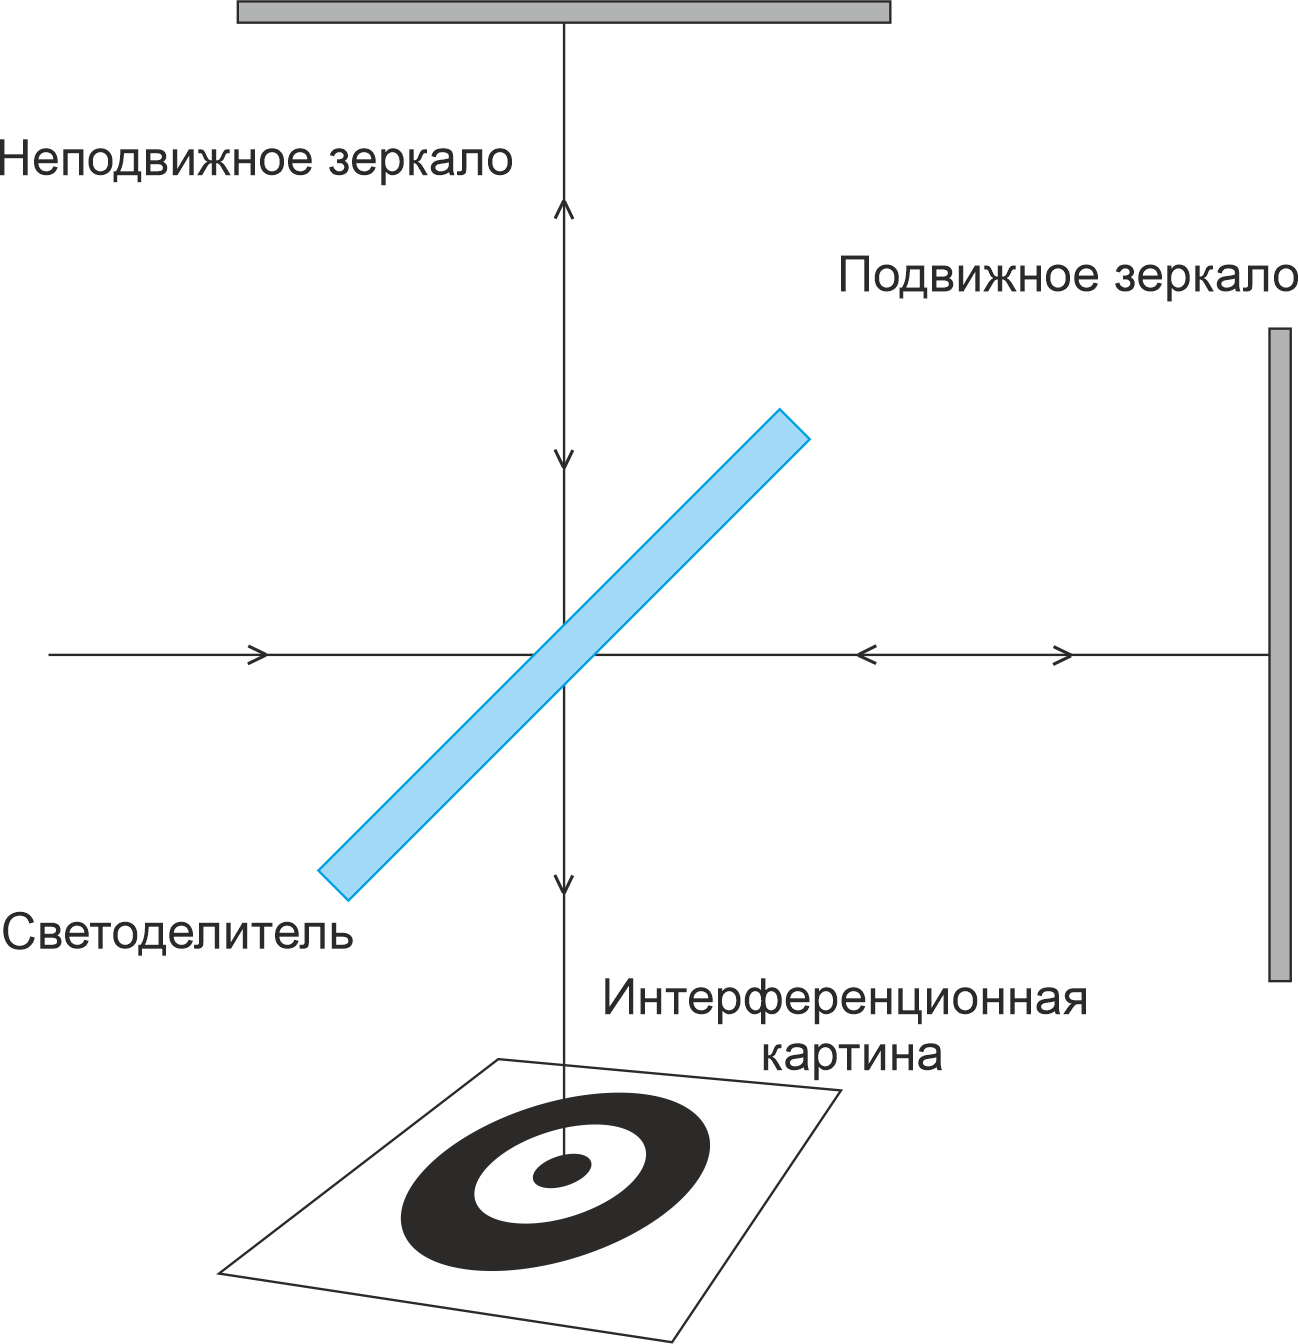
\includegraphics[width=0.5\textwidth]{Mich_int.png}
		\caption{Принципиальная схема интерферометра Майкельсона}
		\label{fig_michelson}
	\end{figure}
	
 Образующими компонентами интерферометра Майкельсона являются подвижное и неподвижное зеркала, светоделитель и детектор, регистрирующий конечную интерференционную картину (рис.~\ref{fig_michelson}). 
	 
 Принцип работы установки заключается в создании контролируемого интерференционного изображения для анализа спектрального состава излучения. Для этого пучок света, поступающий в прибор, разделяется светоделителем на две части. Полученные  компоненты отражаются от зеркал и вновь возвращаются на светоделитель, приобретая разность хода, определяемую перемещением подвижного зеркала. В конечном счете, собранный пучок формирует устойчивую интерференционную картину, считываемую детектором.
 
   	\begin{figure}[h]
   	\centering
   	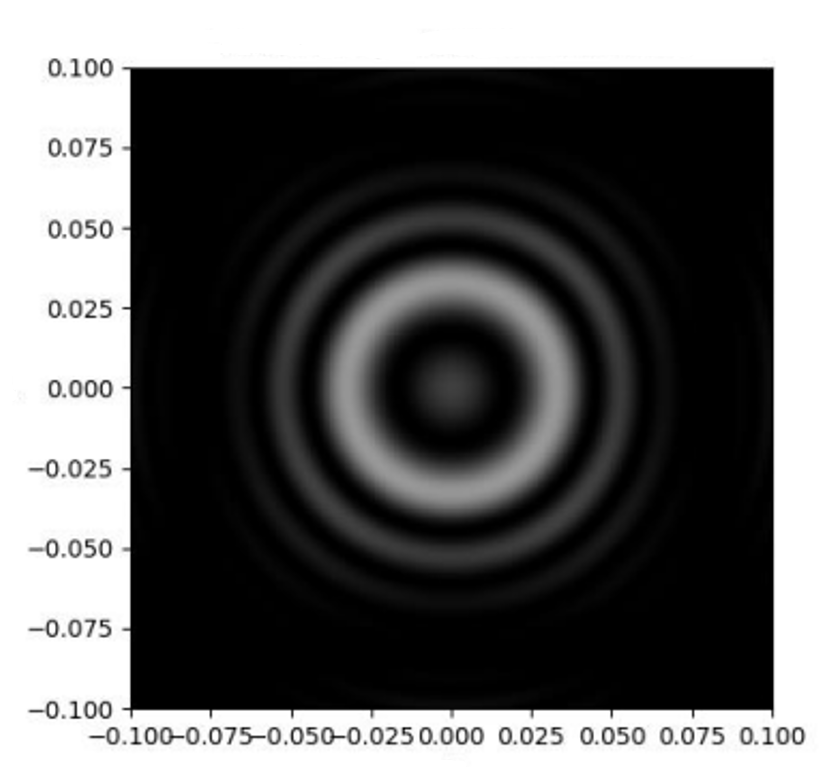
\includegraphics[width=0.5\textwidth]{Intefer_pic.png}
   	\caption{Моделирование интерференционного изображения монохроматического источника}
   	\label{fig_NewtonRings}
   \end{figure}

   Также отметим, что, как правило, источник излучения нельзя считать точечным, поэтому изображение на детекторе при качественной юстировке представляет собой интерференционное кольцо (рис~\ref{fig_NewtonRings}). 
	
	\section{Основное соотношение фурье-спектрометрии}
	
	Зависимость интенсивности излучения на приёмнике от оптической разности хода преобразуется в спектр регистрируемого излучения посредством основного соотношения фурье-спектрометрии \cite{белл1975введение}: 
	\begin{equation}
	 B(\sigma)= \int^{\infty}_{-\infty} \left[ I(\delta)-\frac{1}{2} I(0)\right] e^{-i2\pi\sigma\delta} d\delta,
	 \label{eqn_basicspectro}
	\end{equation}
где $I(\delta)$ - интенсивность, регистрируемая детектором, от оптической разности хода, определяемого положением подвижного зеркала, $B(\sigma)$ - спектральная мощность падающего излучения от изучаемого волнового числа $\sigma$.
	
	Выражение $I(\delta)-\frac{1}{2} I(0)$ в фурье-оптике обозначается $F(\delta)$ и называется интерферограммой. Именно в таком формате передаётся информация с детектора на компьютер для дальнейшей постобработки. Получение интерферограммы с минимальными искажениями за минимальное время является основной задачей при проектировании прибора.
	Отметим, что на практике расчёт интеграла \eqref{eqn_basicspectro} не производится, поскольку вычислительно эффективнее использовать быстрое преобразование Фурье. 
	
\section{Влияние ограниченности оптическая разность хода}

Поскольку база передвижения подвижного зеркала ограничена габаритами прибора, необходимо учитывать их влияние на оптическую разность  хода в регистрируемом спектре. Пусть база подвижного зеркала способна обеспечить оптическую разность хода в диапазоне $[-L,L]$. Тогда интеграл \eqref{eqn_basicspectro} преобразуется как: 
	\begin{equation}
	B(\sigma)= \int^{L}_{-L} \left[ I(\delta)-\frac{1}{2} I(0)\right] e^{-i2\pi\sigma\delta} d\delta
	\label{eqn_basicspectromod}
\end{equation}
Рассмотрим эффект на примере спектра монохроматического точечного источника: $B(\sigma)=\frac{1}{2}\left(\delta'(\sigma-\sigma_0)+\delta'(\sigma+\sigma_0)\right)$. Его интерферограмма, согласно \eqref{eqn_basicspectro}, определяется обратным преобразованием Фурье:
 $$F(\delta)=\int^\infty_{-\infty} \frac{1}{2}\left(\delta'(\sigma-\sigma_0)+\delta'(\sigma+\sigma_0)\right)\cdot e^{i2\pi\sigma\delta} d\sigma= cos(2\pi\sigma_0\delta)$$
 
 \begin{figure}[h]
 	\centering
 	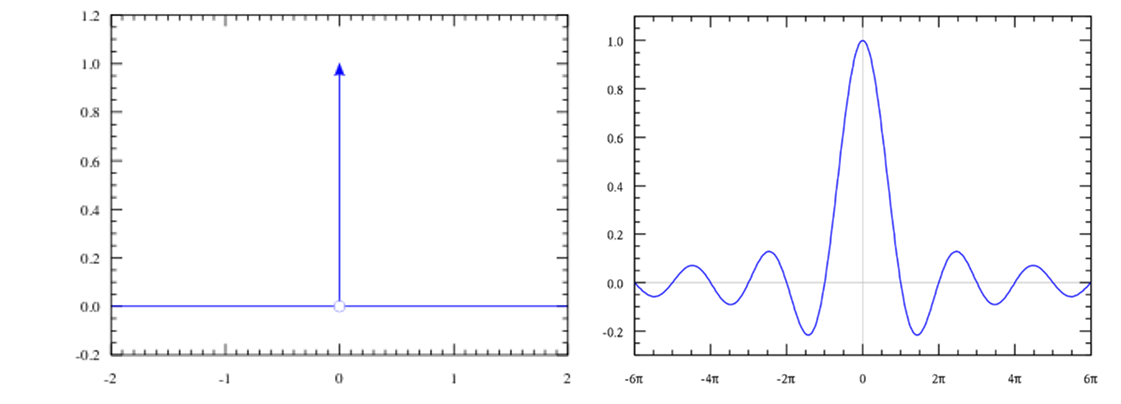
\includegraphics[width=1\textwidth]{Graph.png}
 	\caption{Изменение аппаратной функции прибора в силу ограниченности оптической разности хода}
 	\label{fig_instrumentlimits}
 \end{figure}
 
Регистрируемый прибором спектр при переходе к конечным пределам интегрирования становится равным:
\begin{equation}
 B(\sigma)=\int^L_{-L} cos(2\pi\sigma_0\delta) e^{-i2\pi\sigma\delta} d\delta = 2L \left( sinc\left[2\pi(\sigma_0+\sigma)L\right]+sinc\left[2\pi(\sigma_0-\sigma)L\right] \right)
\end{equation}
Полученный спектр соответствует аппаратной функции (АФ) прибора (рис~\ref{fig_instrumentlimits}). Изменение профиля функции отклика, согласно логике математического анализа, объясняется тем, что базис фурье-преобразования перестаёт быть ортогональным при ограничении спектрального диапазона.

\section{Влияние размера шага дискретизации}
Выражение \eqref{eqn_basicspectro} вводится для бесконечно малого шага подвижного зеркала $d\delta$. На практике же $d\delta$ имеет конечное значение, определяемое числом измерений регистрирующей системы на единицу длины. Таким образом, непрерывный график зависимости интенсивности от разности хода заменяется на дискретный. При этом интеграл \eqref{eqn_basicspectro} при вычислениях также приобретает вид дискретного преобразования Фурье:

\begin{equation}
	B(\sigma)=\sum_{j=-N/2}^{N/2-1} \left[I(j\Delta \delta )-\frac{1}{2}I(0)\right] \cdot e^{-i2\pi \sigma j \Delta \delta}
\end{equation}

Переход к дискретному преобразованию Фурье напрямую связан с определением частоты Найквиста  $\sigma_s=\frac{1}{2\Delta \delta}$.
\begin{figure}[h!]
	\centering
	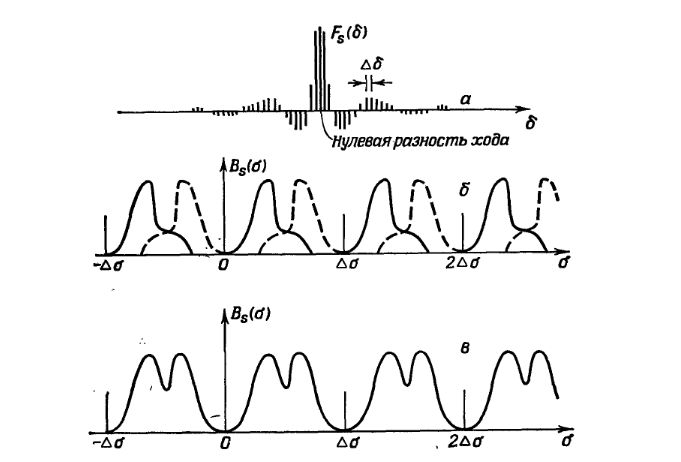
\includegraphics[width=1.\textwidth]{Aliasing.png}
	\caption{a  - дискретная интерферограмма; б - компоненты вычисленного для него спектра; в - полный спектр, который можно вычислить по дискретной интерферограмме}
	\label{fig_aliasing}
\end{figure}

 Согласно теореме Найквиста-Котельникова, в случае, когда непрерывный сигнал имеет спектральное распределение, имеющее ненулевые значения строго в диапазоне волновых чисел $[0,\sigma_s]$, его возможно однозначно восстановить. Следовательно, имеет место взаимное соответствие между спектральным и пространственным представлением сигнала. Если же спектральные компоненты находятся вне полосы Найквиста $[0,\sigma_s]$, то соответствующие гармоники будут искажать сигнал и однозначное восстановление будет невозможно. Такое явление называется алиасингом (aliasing) и эффективно подавляется с помощью низкочастотных оптических и электронных фильтров (рис.~\ref{fig_aliasing}).

\chapter{Технические особенности ФАСТ}
Отдел исследований планет ИКИ имеет значительный опыт построения спектрометров, работающих в ИК, видимом и УФ-диапазонах. В институте были произведены приборы различных габаритов и принципов работы, специфицированные под жесткие условия космических миссий. В этой главе изложена оптическая схема прибора ФАСТ.

\begin{figure}[h]
	\centering
	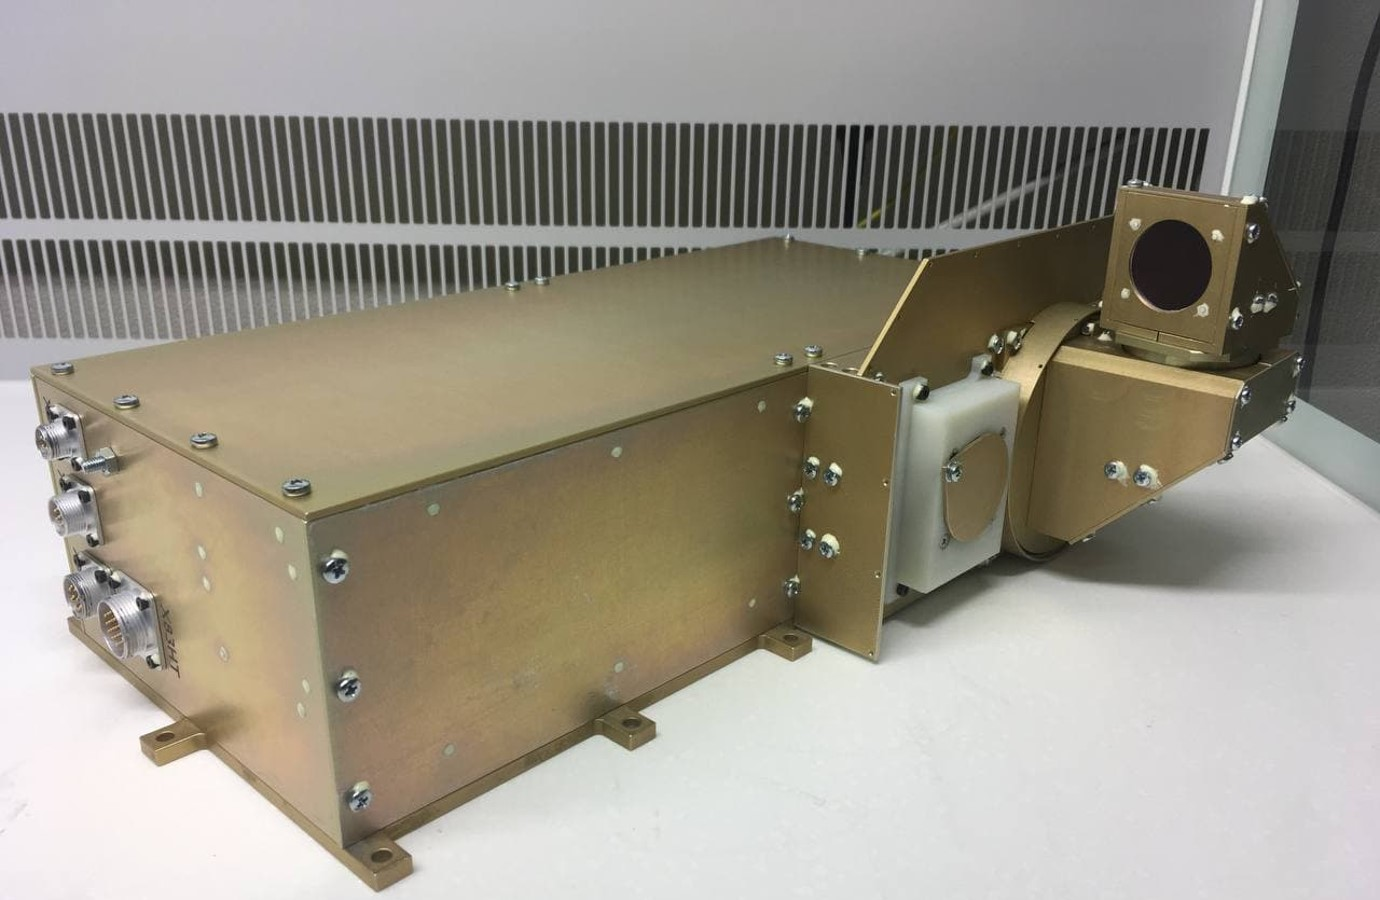
\includegraphics[width=0.9\textwidth]{FAST.jpg}
	\caption{Внешний вид прибора ФАСТ}
	\label{fig_FASTexterior}
\end{figure}
\section{Решаемые задачи и требования к конструкции}

ФАСТ --- спектрометр для исследований атмосферы Марса, работающий в ИК-диапазоне (рис~\ref{fig_FASTexterior}). Среди научных задач, заявленных миссией ''ЭкзоМарс-2022'', ФАСТ выполняет мониторинг температуры и аэрозолей.

 С точки зрения исполнения прибор должен иметь небольшой вес и габариты, устойчив к вибрациям, перепадам температур и внешним электромагнитным полям. Помимо этого специфика работы с оптикой требует микрометрической точности регулировки каждой из компонент.


\begin{figure}[h!]
	\centering
	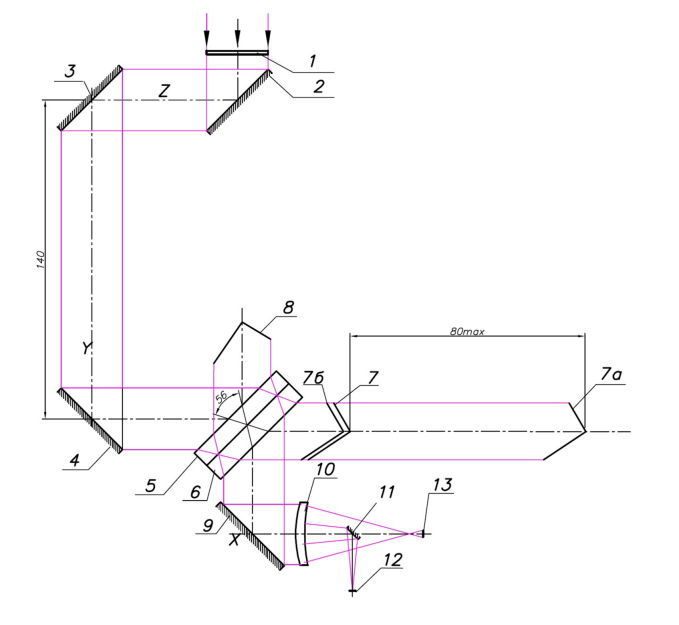
\includegraphics[width=0.9\textwidth]{Scheme.png}
	\caption{Оптическая схема ФАСТ. (1)—входное
		окно (Ge); (2), (3), (4), (9) и (11) — плоские зеркала; (5)—компенсатор (KBr);
		(6)—светоделитель (KBr); (7),
		(8)—угловые отражатели;
		(10)—асферическая линза ZnSe; (12)—
		светочувтсвительная матрица (32 × 32);
		(13)—пиродетектор. (7a)
		и (7b) — граничные положения
		подвижного уголкового отражателя}
	\label{fig_FASToptical}
\end{figure}


Согласно техническому заданию основные параметры и характеристики прибора задаются следующими значениями \cite{shakun2017fourier}:
\begin{itemize}
	\item вес: 3.5 кг;
	\item спектральный диапазон: 1.7-17 микрон / 500-5000 $см^{-1}$; 
	\item спектральное разрешение: 1 $см^{-1}$.
\end{itemize}

Данные требования вызывали необходимость модификации, определяющую конструкцию прибора (рис.~\ref{fig_FASToptical}). 




\section{Референтный канал}
	
	Для отслеживания оптической разности хода используется реферетный канал. Система обеспечивает большую точность дискретизации и работу в широком спектральном диапазоне. 
	
	Принцип работы референтного канала основан на интерференции разделенных пучков. Приёмник референтного сигнала регистрирует излучение DFB-лазера, проходящего оптический путь идентичный пути входного сигнала. При фиксации зануления на детекторе референтного сигнала в результате итерференции, управляющая система прибора получает сигнал о начале нового шага дискретизации. Таким образом, отсчёты выполняются при перемещении подвижного зеркала на половину длины волны опорного лазера.   
	
	\section{Уголковые отражатели}
	
	Для упрощения юстировки оптической системы интерферометра в схеме используются уголковые отражатели с секундной точностью (рис.~\ref{fig_reflectors}). За счёт фиксированного угла раствора между отражающими поверхностями уголок обеспечивает параллельность падающего и выходящего светового пучка с высокой точностью. Это свойство определяет основное преимущество уголковых отражателей перед плоскими зеркалами: регулировка положения оптического элемента происходит не по угловой степени свободы, а по поступательной. Благодаря этому, возможна более тонкая и устойчивая к внешним воздействиям настройка прибора. В реализации ФАСТ замена плоских зеркал на уголковые отражатели привела к кратному выигрышу в чувствительности юстировки.
	
	\begin{figure}[h!]
		\centering
		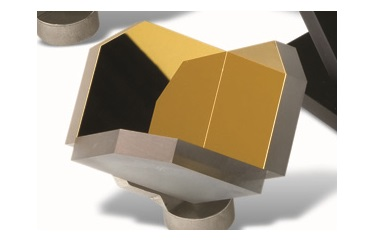
\includegraphics[width=0.6\textwidth]{Corn_ref.jpg}
		\caption{Уголковые отражатели}
		\label{fig_reflectors}
	\end{figure}
	
	\section{Материал оптических элементов}
	
 Выбор материала оптических элементов схемы зависит от изучаемого спектрального диапазона. Наиболее важен выбор материалов светоделителя и светофильтра.
	
	\begin{figure}[h]
		\centering
		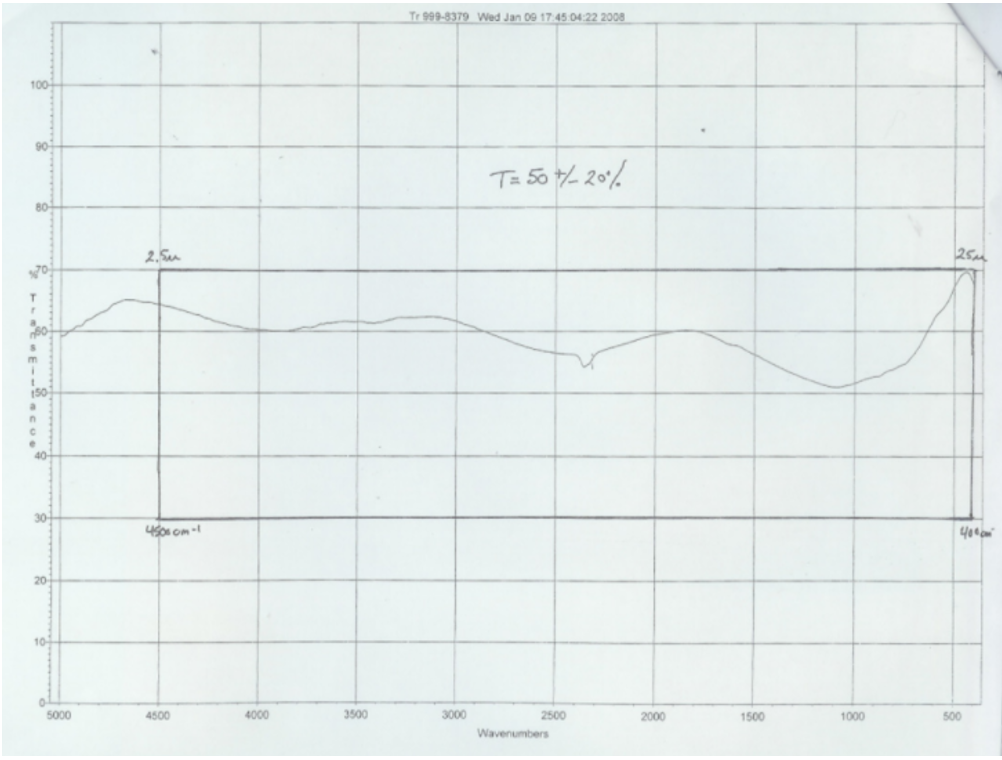
\includegraphics[width=0.7\textwidth]{KBR.png}
		\caption{Кривая зависимости показателя энергетического отражения светоделителя в диапазоне 500-5000 $см^{-1}$}
		\label{fig_lightcurve}
	\end{figure}
	
	В реализации ФАСТ входное окно, фильтрующее спектральные компоненты падающего излучения, выполнено из германия, имеющего известную проницаемость в диапазоне 1.7-17 мкм и поглощающего при больших частотах. При ограниченном запасе в шаге дискретизации, такой фильтр с хорошей точностью ограничивает сигнал в полосе Найквиста, что позволяет подавить алиасинг.  Для светоделителя используется KBr и специальное многослойное оптическое покрытие, совместно задающие показатель энергетического отражения в районе 50\% на изучаемом диапазоне (рис.~\ref{fig_lightcurve}). 
	
	\section{Детектор}
	
  Интерференционная картина в ФАСТ регистрируется пиродетектором. Его габариты соответствуют наименьшему наблюдаемому интерференционному кольцу. Таким образом, обеспечивается максимальное разрешение при заданной апертуре. Уменьшение площади детектора сопровождается снижением шумового сигнала пропорционального его линейному размеру.
  
   Для оценки качества работы детектора используют удельную обнаружительную способность к обнаружению $D^*$. Величина определяет минимальное значение возможного для регистрации полезного сигнала.  Пиродектор ФАСТ имеет $D^*=2.5 \cdot 10^{9}$ $см Гц^{\frac{1}{2}} Вт^{-1}$. Заданное значение обеспечивает возможность мониторинга яркостных температур и аэрозолей.
	
	\section{Cистема наведения}
	
	Для оптических схем важно, чтобы главная оптическая ось прибора совпадала с центром источника излучения. Это позволяет минимизировать влияние пространственной некогерентности излучения. Для этих целей часть падающего излучения после прохождения светоделителя  отводится небольшим зеркалом на светочувствительную матрицу. Формируемое на ней изображение определяет распределение интенсивностей на входном окне. Это позволяет судить о расположении источника света в пространстве. При наличии отклонений положение подвижной зрительной трубы прибора корректируется с точностью до пикселя матрицы с помощью разработанного алгоритма. Механическая свобода перемещения входного окна обеспечивается шкивами, способными с точностью до 0.1 мрад задавать направления наблюдения на небесной полусфере.  \cite{shakun2019two}.
	
	\begin{figure}[h]
		\centering
		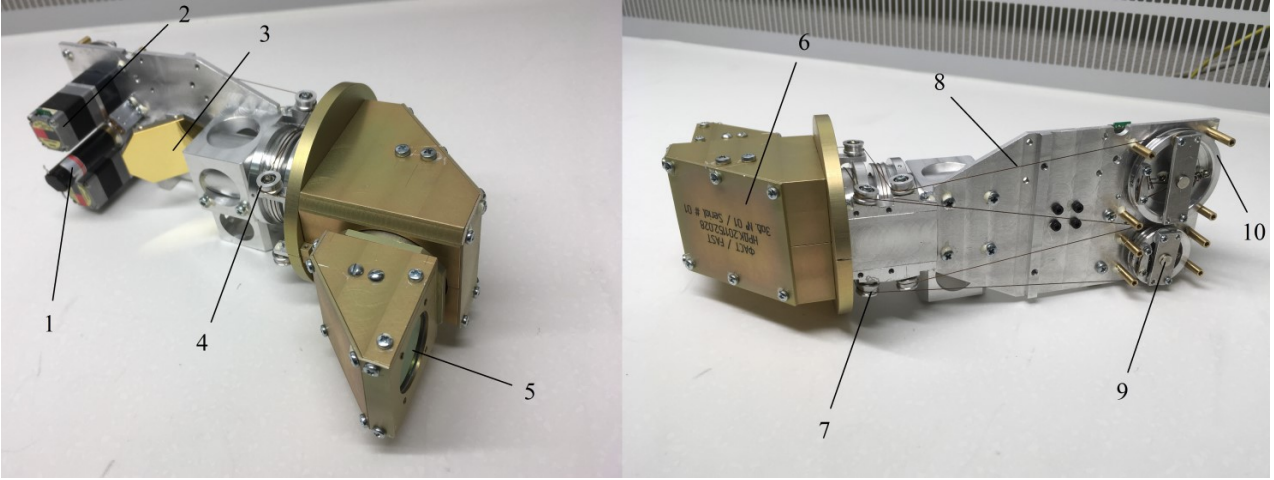
\includegraphics[width=\textwidth]{Scanner.png}
		\caption{Система наведения ФАСТ. (1) механизм блокировки; (2) шаговый двигатель с зубчатой передачей; (3) закрепленное плоское
			зеркало; (4) и (7) шкивы; (5) входное окно (Ge); (6) защитный кожух; (8) стальной трос; (9) магнит главного шкива; (10) главный шкив с магнитным энкодером}
		\label{Scanner}
	\end{figure} 
	 
	
	\section{Черные тела}
	
	Калибровку интерферометра Майкельсона удобно проводить на черных телах. Их спектр непрерывен и задаётся аналитически, что значительно упрощает вычислительную обработку. С другой стороны, на рынке технического оборудования существует большое количество реализаций черных тел разных габаритов и мощностей. Также существенным преимуществом является доступность черных тел в освоении и эксплуатации. 
	
	Внутренее черное тело ФАСТ компактно (60x75x70 $мм^3$), изменяет температуру в диапазоне $20^\circ C$, покрывает входную апертуру прибора и имеет степень черноты $\epsilon \approx 0.995$.  \cite{shakun2019compact,} 




		
	\chapter{Радиометрическая калибровка}
	
	Для качественного восстановления спектра внешнего излучения необходимо проводить калибровку прибора.  Процедура заключается в измерении спектров черных тел с известными характеристиками для получения соответствия между энергетической яркостью источника и показаниями приёмника. 

Принципиально разделять полевую и лабораторную калибровку приборов, так как эти процессы имеют индивидуальные особенности. 

Лабораторные измерения, как правило, проводятся однократно с большой точностью для верификации заявленных технических возможностей прибора. Высокое качество таких исследований объясняется тем, что в лабораторных условиях возможно проводить длительные эксперименты с габаритным оборудованием, позволяющим тщательно изучить поведение прибора в различных режимах работы. 
 
 Необходимость проведения полевой калибровки связана с изменением восприимчивости прибора к внешнему излучению с течением времени. Возможными причинами изменений свойств прибора могут быть запыление входного окна, разъюстировка оптической схемы и сбои в работе электроники. Это приводит к серьезным ошибкам определения спектра. Таким образом, основной задачей полевой калибровки является отслеживание изменений и своевременная корректировка кривых восприимчивости.
	
	\section{Линейное приближение}
	
	Считая, что показания прибора и интенсивность падающего излучения линейно связаны, получим:
		\begin{equation}
С_\nu(\nu,T)=r_\nu(\nu)\cdot\left(B_{target}(\nu,T)-B_{inst}(\nu,T_{inst})\right) \cdot e^{i\phi_1(\nu)}, 	
	\end{equation}
где $С_\nu(\nu,T)$ - фиксируемое детектором излучение (в битах), $r_v$  - относительная восприимчивость прибора, $\phi_1$ - фазовая восприимчивость прибора, $B_{inst}$   - излучение, исходящее от приёмника и корпуса прибора (в $\frac{Дж}{см^2 \cdot c \cdot стеррад}$), $B_{target}$  - излучение, исходящее от изучаемого источника (в $\frac{Дж}{см^2 \cdot c \cdot стеррад}$). 

Используемое предположение о линейности как правило справедливо для большинство детекторов, и его возможно проверить построив статистическую гипотезу о наличии нелинейного члена.
	
	\section{Радиометрическая калибровка}
	
В статье \cite{revercomb1988radiometric} описан более точный способ восстановления спектра. Автор указывает на необходимость учета возможности когерентного переотражения излучения приёмника от светоделителя. Таким образом, в итоговой формуле вводится член, определяющий разность фаз между регистрируемым и приборным излучением.

\begin{equation}
	С_\nu(\nu,T)=r_\nu(\nu)\cdot\left(B_{target}(\nu,T)+B_{inst}(\nu,T_{inst})\cdot e^{i\phi_2(\nu)}\right) \cdot e^{i\phi_1(\nu)}
	\label{eqn_phaseterm}
\end{equation}

Рассмотрим процедуру восстановления спектра неизвестного источника $B_{goal}$ по измерениям прибора. Если принять, что известны результаты калибровки на черном теле при температурах $T_1$ и $T_2$ при фиксированной инструментальной температуре $T_{inst}$:   
\begin{equation}
\left\{\begin{array}{l}
	C_{T_1}=r_\nu \cdot \left(B_{BB}(T_1)+B_{inst}(T_{inst})\cdot e^{i\phi_2(\nu)}\right) \cdot e^{i\phi_1(\nu)}\\
	 C_{T_2}=r_\nu \cdot \left(B_{BB}(T_2)+B_{inst}(T_{inst})\cdot e^{i\phi_2(\nu)}\right) \cdot e^{i\phi_1(\nu)}\\
 	 C_{goal}=r_\nu \cdot \left(B_{goal}+B_{inst}(T_{inst})\cdot e^{i\phi_2(\nu)}\right) \cdot e^{i\phi_1(\nu)}
\end{array}\right.	
\end{equation}
Выражая $B_{goal}$, получим:
\begin{equation}
(С_{goal}-С_{T_1}) \cdot \frac{B_{BB}(T_1)-B_{BB}(T_2)}{C_{T_1}-C_{T_2}}+B_{BB}(T_1)=B_{goal}
\end{equation}
Результат можно улучшить, усреднив спектры калибруемых тел, тем самым исключив случайную ошибку:
\begin{equation}
	(С_{goal}-<С_{T_1}>) \cdot \frac{B_{BB}(T_1)-B_{BB}(T_2)}{<C_{T_1}>-<C_{T_2}>}+B_{BB}(T_1)=B_{goal} 
	\label{eqn_bgoal}
\end{equation}

	\section{Precise Dual Phase Calibration (PDPC)}
	
	В ходе эксперимента температура прибора и калибровочного черного тела могут изменяться от измерения к измерению (рис.~\ref{fig_tempdrift}). То есть $T_1,T_2,T_{inst}$ нельзя считать постоянными на протяжении эксперимента. Следовательно, усреднение спектров как в \eqref{eqn_bgoal} уже не представляется возможным. Для устранения случайной ошибки в этом случае требуется разработка более совершенного метода.
	
	\begin{figure}[h]
		\centering
		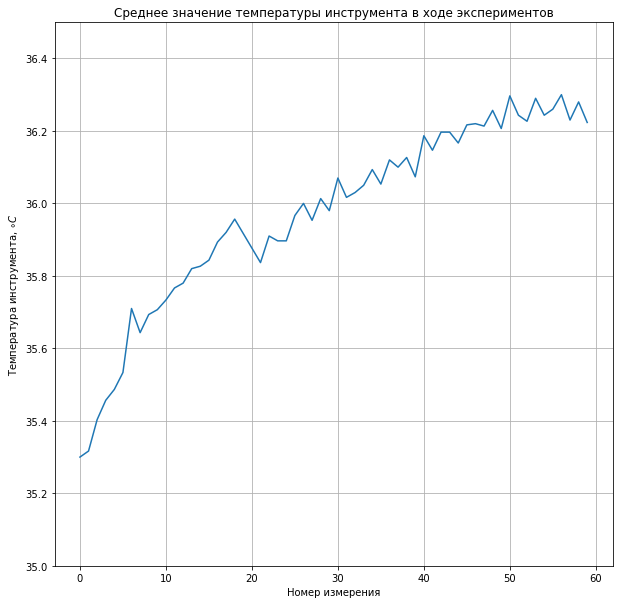
\includegraphics[width=0.6\textwidth]{Temp_bad.png}
		\caption{Пример значительного изменения температуры инструмента за время эксперимента}
		\label{fig_tempdrift}
	\end{figure}

	Для этих целей необходимо выделить в \eqref{eqn_phaseterm} члены не зависящие от изменений в температурах. Это абсолютная, нормальная и аномальная фазовая восприимчивость. Запишем систему уравнений, соответствующие $N$ измерениям: 
	\begin{equation}
		\left\{\begin{array}{l}
			C_{T_1}=r_\nu \cdot \left(B_{BB}(T_1)+B_{inst}(T_{inst_1})\cdot e^{i\phi_2(\nu)}\right) \cdot e^{i\phi_1(\nu)}\\
			C_{T_2}=r_\nu \cdot \left(B_{BB}(T_2)+B_{inst}(T_{inst_2})\cdot e^{i\phi_2(\nu)}\right) \cdot e^{i\phi_1(\nu)}\\
			...\\
			C_{T_N}=r_\nu \cdot \left(B_{BB}(T_N)+B_{inst}(T_{inst_N})\cdot e^{i\phi_2(\nu)}\right) \cdot e^{i\phi_1(\nu)}
		\end{array}\right.	
	\end{equation}
	Заметим, что если каждое \(i\)-ое уравнение разделить на соответствующий $B_{inst}(T_{inst_i})$, то система принципиально сводится к задаче линейной регрессии с единственным параметром и свободным членом:
\begin{equation}
	Y=k(\nu) \cdot X + \beta(\nu),
	\label{eqn_objective}
\end{equation}
 где $k$ и $\beta$ - комплексные функции, зависящие только от волнового числа $\nu$, а \(X\) и \(Y\) - векторы действительных чисел с числом элементов \(N\).

	Техника PDPC предполагает применение МНК для нахождения коэффициентов модели \eqref{eqn_objective} при каждом заданном волновом числе. Таким образом, находится среднее значение восприимчивости для набора наблюдений, что в значительной степени подавляет случайную ошибку.
	
	\begin{figure}[h]
		\centering
		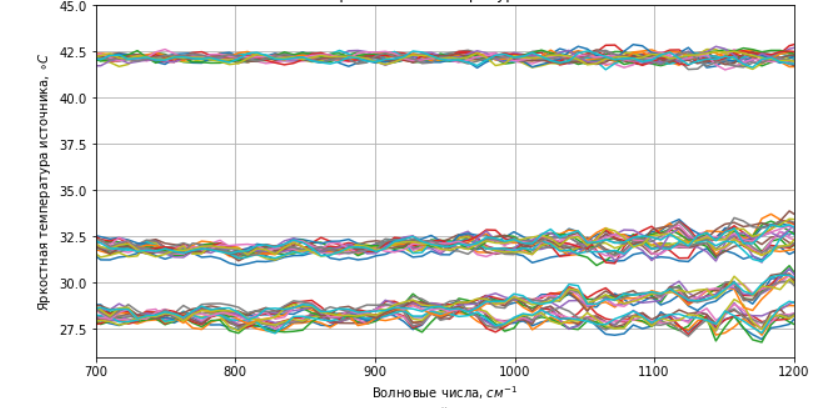
\includegraphics[width=\textwidth]{PDPC.jpg}
		\caption{График яркостных температур при применении техники PDPC}
		\label{fig_PDCtemps}
	\end{figure}
	
	PDPC отличает устойчивость температурного профиля в широком диапазоне частот (рис.~\ref{fig_PDCtemps}), возможность работать в условиях, при которых точная температурная стабилизация невозможна.
	
	\section{Double Precision Dual Phase Calibration (DPDPC)} \label{sec_DPDPC}
	
	Техника DPDPC используется в случае, если характерное время изменения инструментальной температуры сравнимо с временем записи интерферограммы $t_{measurement}$. То есть:
	$$dt/dT \cdot \Delta T \sim t_{measurement},$$
	 где $\Delta T$ - задаваемая точность измерений температуры. 
	
	В этом случае необходимо учитывать, что интерферограмма в каждой точке дискретизации записывалась для различных температур. Используя теорему Лагранжа, в предположении что исходный спектр дифференцируем, получаем:
	$$ B(T(x),\nu)=\underset{спектр\ при\ T=const}{B(T(0),\nu)}+\underset{аномальный\ член}{B'_T(T(\xi),\nu)T'_x(\xi) \cdot x},$$
	где $\xi$ находится на интервале \(\left[0;x\right]\).
	
	Для оценки влияния аномального члена сверху возьмем максимальный по модулю наклон прямой за время записи: $k(\nu)= \underset{x \in [-L,L]}{max} \left| B'_T(T(x),\nu)T'_x(x) \right| $.
	
	Таким образом, получим выражение для интерферограммы аномального члена спектра:
	\begin{equation}
		F_{anom}(\delta)=  \int^{\infty}_{-\infty} k(\nu)\cdot \delta \cdot exp(i 2 \pi \nu \delta) d\nu
	\end{equation}
	В этом случае, согласно \eqref{eqn_basicspectromod}, считываемый спектр запишется как:
	\begin{equation}
		\begin{split}
			B_{anom}(\sigma) = \int^{L}_{-L} F_{anom}(\delta) \cdot exp(i 2 \pi \sigma \delta) d\delta =  \int^{L}_{-L}\int^{\infty}_{-\infty} k(\nu)\cdot \delta \cdot exp(i 2 \pi (\sigma-\nu) \delta) d\sigma d\nu \\ = \int^{\infty}_{-\infty} k(\nu)  \cdot 2iL^2 \cdot \frac{sinc(L(\sigma-\nu))-cos(L(\sigma-\nu))}{L(\sigma-\nu)} d\nu
		\end{split}
	\end{equation}
 Таким образом, аномальная компонента спектра задаётся сверткой производной нормальной части спектра с функцией отклика вида $AF_{anom}=2iL^2\frac{sinc(Lx)-cos(Lx)}{Lx}$. Используя выражение $k(\nu)$, получаем итоговую формулу:
\begin{equation}
	B_{anom} (\sigma) \approx \underset{x \in [-L,L]}{max}T'_x \cdot (AF_{anom} \ast B'_{norm})(\sigma) 
\end{equation}
  
  	\begin{figure}[h]
  	\centering
  	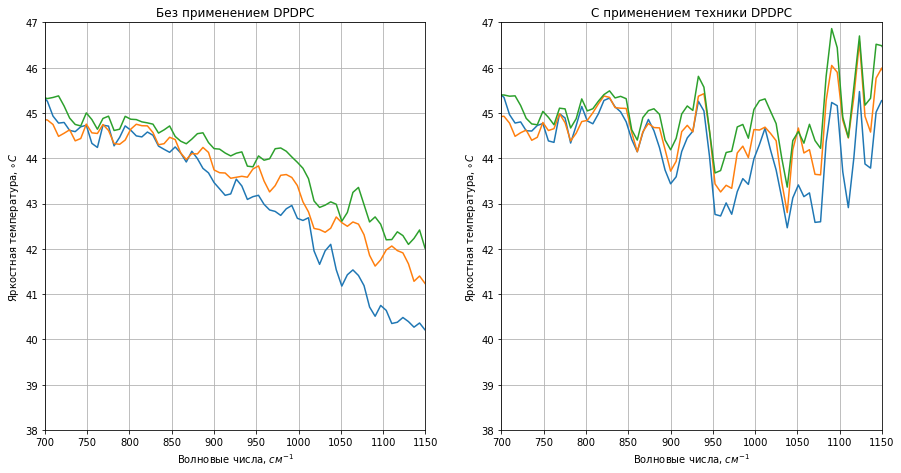
\includegraphics[width=1\textwidth]{DPDPC.png}
  	\caption{Коррекция графика яркостных температур калибровочного тела с температурой $T_{calibr}=45^\circ C$ с помощью техники DPDPC}
  	\label{fig_tempcorr}
  \end{figure}
  
  	DPDPC позволяет производить коррекцию температурного профиля в условиях значительного перепада температур при регистрации интерферограммы. Обратимся к примеру на рис.~\ref{fig_tempcorr}. Несмотря на то, что конечный результат всё также в значительной степени зашумлён, техника позволяет исключить нисходящий линейный тренд --- систематическую ошибку, возникающую вследствие нагрева прибора.
  	
	\chapter{Эксперимент}
	
	Для определения и верификации характеристик прибора был проведён ряд лабораторных испытаний:
	\begin{itemize}
		\item измерение аппаратной функции; 
		\item верификация подградусной точности измерения яркостной температуры;
		\item определение чувствительности прибора;
		\item оценка характерного времени температурного установления.
	\end{itemize}

В каждом из следующих разделов будет приведено описание эксперимента и выводы, полученные в результате обработки.
	\section{Измерение аппаратной функции}	
	Экспериментальная установка имеет следующую конфигурацию:
\begin{figure}[h!]
	\centering
	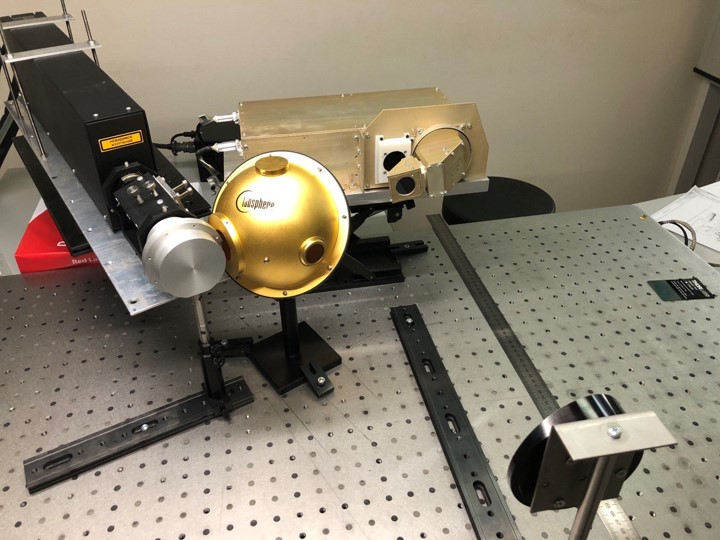
\includegraphics[width=0.65\textwidth]{Laser_exp.jpg}
	\caption{Схема эксперимента по измерению аппаратной функции прибора}
\end{figure}

Лазерный пучок с рабочей длиной волны 632.8 нм, посредством интегрирующих сфер, коллимируется в тонкий, параллельно текущий поток излучения, поступающий на входное окно ФАСТ. Для юстировки схемы используется внеосевое параболическое зеркало, позволяющее с достаточной точностью регулировать направление хода излучения. После прохождения всех оптических элементов прибора излучение лазера собирается на детекторе для формирования интерференционного изображения, которое регистрируется при различных разностях хода. Полученные данные записываются в интерферограмму, выполняемую при максимальной доступной разности оптического хода. Поскольку уширение спектральной линии лазера крайне мало, то полученный спектр можно считать аппаратной функцией прибора.

Всего в ходе эксперимента было зарегистрировано 10 интерферограмм, полученных при различных положения лазерного пятна на детекторе. Финальный вид аппаратной функции был установлен по максимальному значению интенсивности, соответствующему наименьшему удалению пути лазерного пучка от оптической оси прибора.

	\begin{figure}[h]
	\centering
	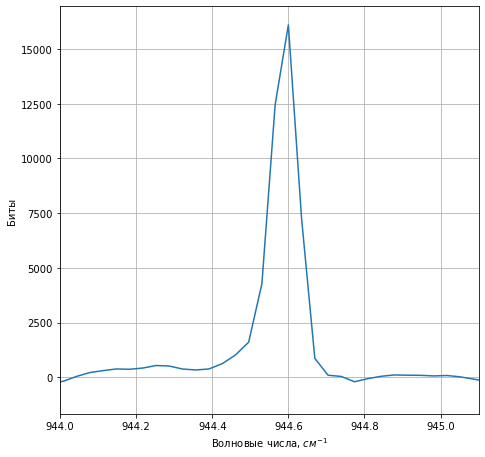
\includegraphics[width=0.6\textwidth]{AF.png}
	\caption{Аппаратная функция ФАСТ. FWHM $\approx 0.05 см^{-1}$}
\end{figure}

Исходя из экспериментально полученного значения полуширины аппаратной функции, можно сделать вывод, что прибор способен обеспечивать спектральное разрешение до $0.05 см^{-1}$. 

	\section{Верификация подградусной точности измерения яркостной температуры}
	Одной из поставленных перед конструкторами ФАСТ задач было обеспечение подградусной точности измерения яркостной температуры. Для верификации достижения этой цели был поставлен эксперимент по измерению априорно известного спектра черного тела. Кривую восприимчивости, аналогично полевому эксперименту, предполагалось получить из наблюдений внутренних черных тел.
	
	Для этого прибор в начале эксперимента провёл 20 измерений внутреннего черного тела при температуре $29^\circ С$ и $32^\circ С$. По полученным интерферограммам была построена функция восприимчивости ФАСТ (рис.~\ref{fig_FASTsuscept}). Для этого была использована техника PDPC, поскольку в ходе эксперимента температура прибора плавно увеличилась на $2^\circ С$.
	
   \begin{figure}[h!]
		\centering
		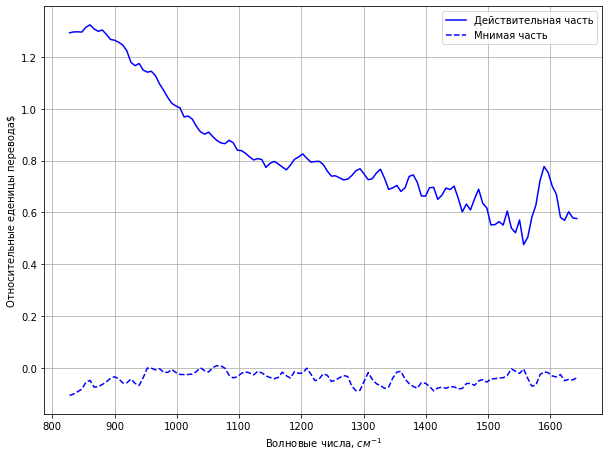
\includegraphics[width=0.7\textwidth]{Response.png}
		\caption{Функция восприимчивости ФАСТ}
		\label{fig_FASTsuscept}
	\end{figure}
	
	В ходе второй части эксперимента были выполнены 40 измерений внешнего черного тела при температуре $47^\circ С$. Полученные из калибровки яркостные температуры измеряемых тел были нанесены на общий график, позволяющий судить о высоком качестве проведенного эксперимента.
	
		\begin{figure}[h!]
		\centering
		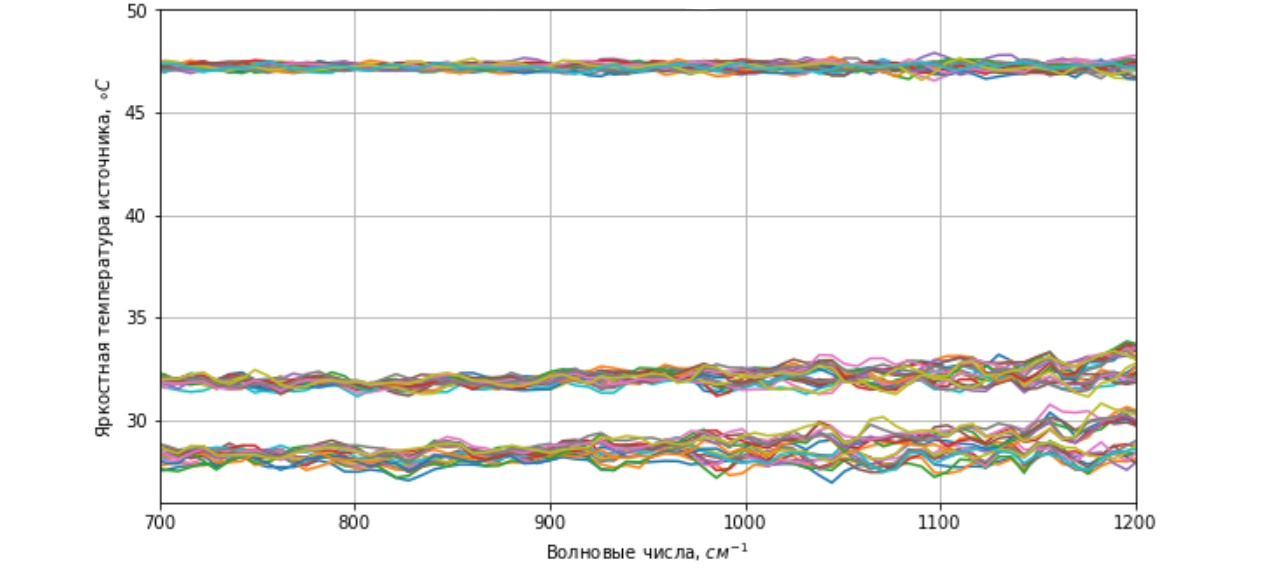
\includegraphics[width=\textwidth]{PDPC_exp.jpg}
		\caption{График яркостных температур в эксперименте }
		\label{fig_brightexp}
	\end{figure}
	
	
	Отметим, что наличие биений в графиках измерений яркостных температур внутренних черных тел в районе 1000 $см^{-1}$ связано с разностью обработки электронным фильтром интерферограммы вправо и влево (рис.~\ref{fig_brightexp}). При их усреднении ошибка в линейном приближении компенсируется.
	
		
Таким образом, в результате эксперимента установлено соответствие между температурой калибровочного тела и его наблюдаемой яркостной температурой с точностью не хуже $1^\circ$C. Это подтверждает заявленные технические характеристики прибора.

	\section{Чувствительность прибора}
	
	Результаты предыдущего эксперимента также позволяют оценить чувствительность прибора. В радиометрии для количественного анализа способности спектрометра выделять полезный сигнал из шума используются два параметра: NESR (Noise Equivalent Spectral Radiance) и SNR (Signal Noise Ratio). 
	
	SNR рассчитывается как отношение полезного сигнала к шуму. Спектры с высокими значениями SNR позволяют достоверно измерять концентрацию поглощающего вещества. NESR определяет величину порогового значения входного сигнала, при котором SNR=1. Если изучаемое излучение меньше NESR, то зашумленность будет превышать полезный сигнал. 
	
	\begin{figure}[h!]
		\centering
		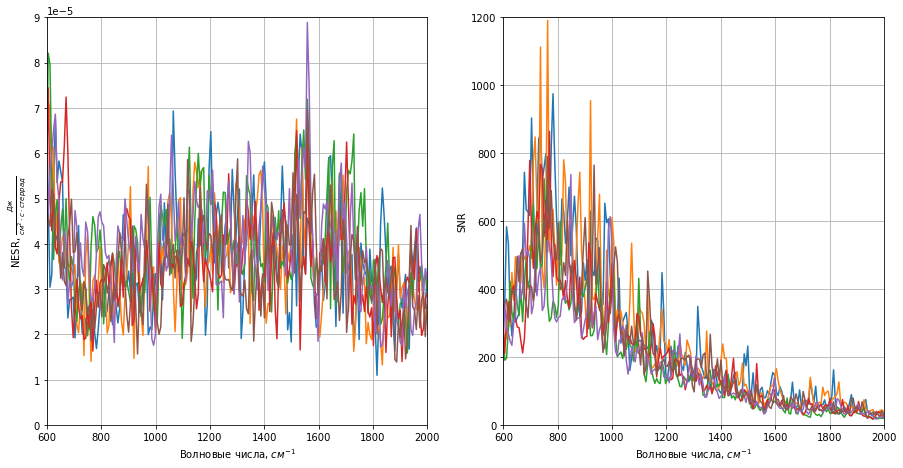
\includegraphics[width=\textwidth]{NESR.png}
		\caption{Графики NESR и SNR экспериментальных данных}
		\label{NESR}
	\end{figure}
	
	
	Для оценки величины шума в экспериментальных данных рассчитывается стандартное отклонение измерений при фиксированной температуре калибровочного тела. За полезный сигнал принимается среднее арифметическое спектров. Таким образом, производится оценка NESR и SNR в условиях лабораторного эксперимента (рис.~\ref{NESR}).
	
	Анализ показывает стабильное значение NESR в спектральном диапазоне 600-2000 $см^{-1}$. Уровень шума позволяет фиксировать спектр черного тела и линии поглощения аэрозолей (SNR > 100). Малые составляющие требуют большего порядка точности и в условиях полевого эксперимента не могут быть зарегестрированы ФАСТом.   

	\section{Оценка характерного времени температурного установления}
	
	 В отсутствие наблюдений прибор для экономии энергии отключается от электропитания. Вследствие этого температура ФАСТ сравнивается с температурой среды. При подключении питания, в результате джоулевых и механических потерь, прибор нагревается, что может негативно сказываться на качестве интерферограммы. Следует определить характерное время, за которое ФАСТ достигнет стабильной температуры. Для этого построим простейшее модельное уравнение:
	 $$C \frac{dT}{dt}=-\kappa(T-T_c)+P,$$
	где $T$ - температура прибора, $T_c$ - температура среды, $P$ - мощность источника тепла, $\kappa$ - константа теплообмена прибора со средой. 
	
	Считая $T(0)=T_c$, получаем:
	\begin{equation}
	T=T_c+\frac{P}{\kappa} \left(1-e^{-\frac{\kappa}{C}t}\right) 
	\end{equation}

	Таким образом, возрастание температуры происходит по закону $1-e^{-t/\tau}$, где характерное время нагревания $\tau$ задаётся параметрами среды и прибора.

	
	Для постановки эксперимента были проведены 60 измерений внешнего черного тела при температуре $45^\circ C$ по мере нагревания прибора. Инструментальная температура измерялась системой датчиков, расположенных по периметру ФАСТ  (рис.~\ref{fig_modeldata}).
	 
	 Данные телеметрии с хорошей точностью подтверждают предложенную модель. Исходя из метода наименьших квадратов, находим, что  характерное время температурного установления примерно равно 19 минутам.


	
	Как было показано в разделе \ref{sec_DPDPC} изменение температуры инструмента приводит к появлению нисходящего линейного тренда при измерении спектра черного тела. Этот факт позволяет оценить характерное время нагрева, по изменению наклона спектров.
	
		\begin{figure}[h!]
		\centering
		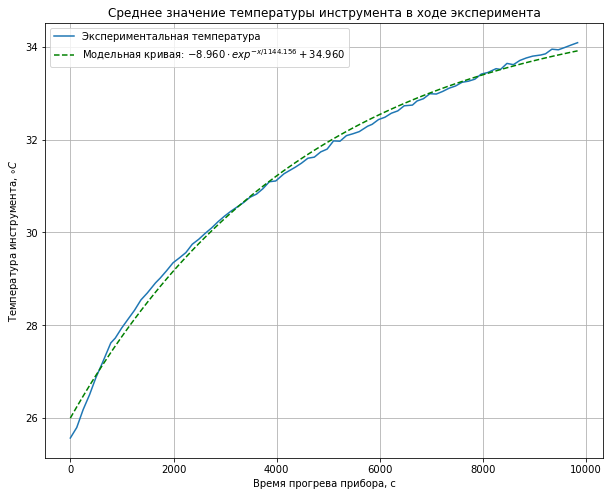
\includegraphics[width=0.75\textwidth]{Model+exp.png}
		\caption{Описание модельных данных экспериментальной кривой}
		\label{fig_modeldata}
	\end{figure}
	
 Определив с помощью МНК (рис.17) коэффициенты линейной регрессии для каждого измерения, получаем что за 12 итераций наклон кривой изменился в $e$ раз. Отсюда, исходя из средней продолжительности измерения в 104 секунды, находим, что $T_{стаблизации}$ равно 20 минутам. Таким образом, измерения характерного времени температурной стабилизации посредством двух различных подходов с хорошей точностью совпадают, что позволяет судить об адекватности полученного результата.  
 
 	\begin{figure}[h!]
 	\centering
 	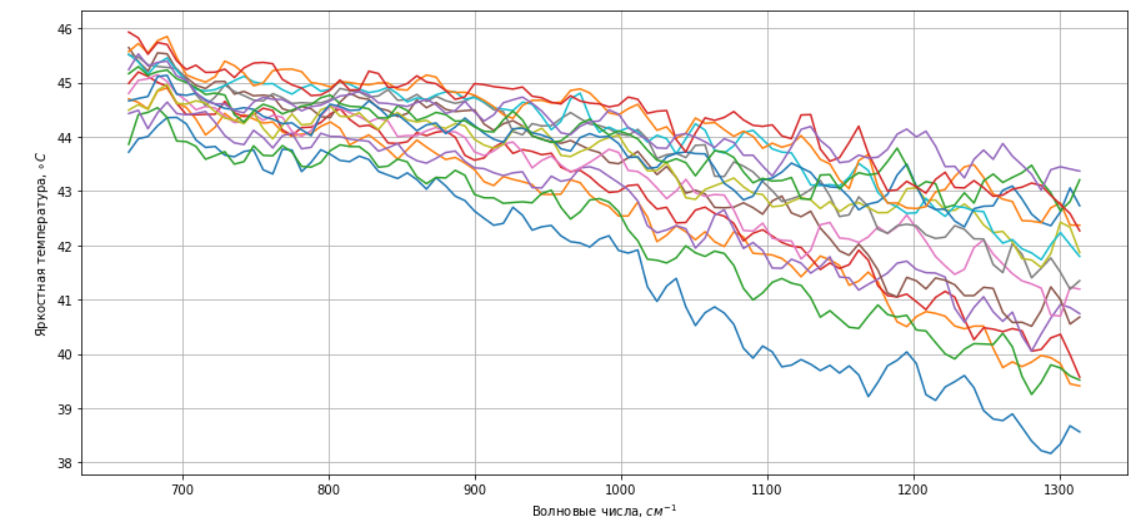
\includegraphics[width=1\textwidth]{Progrev.png}
 	\caption{Изменение графика яркостной температуры по мере прогревания прибора}
 \end{figure}
	
\chapter{Заключение}

	Для калибровки лабораторного эксперимента были освоены существующие и разработаны новые методы, позволяющие нивелировать систематические ошибки в отсутствие термической стабилизации. Предложенные методы могут иметь практическое приложение в условиях полевого эксперимента. В частности, метод DPDPC позволяет использовать время прогрева прибора для предварительной оценки спектра окружающей среды.  

 	В работе также описана постановка экспериментов, выполненных с целью исследования характеристик прибора. Каждый эксперимент покрывает один из ключевых параметров ФАСТ: функцию восприимчивости, время температурной стабилизации, восприимчивость спектрометра, ширину аппаратной функции. Таким образом, были верифицированы заявленные технические характеристики прибора: максимальное спектральное разрешение до 0.05 $см^{-1}$, подградусная точность измерения яркостной температуры, разрешение линий поглощения аэрозолей. Это позволяет заключить, что прибор готов для выполнения поставленных космических задач.
 	
	 Помимо этого представлено описание модификаций конструкции ФАСТ. Описаны принципы работы системы высокоточной навигации поля зрения прибора по небесной сфере и референтного канала дискретизации, обеспечивающего работу в широком спектральном диапазоне. Также изложены и прокомментированы решения, принятые относительно выбора оптических элементов и организации схемы спектрометра. 

\emph{Настоящая работа выполнена в Институте Космических Исследования РАН. Автор благодарит своего научного руководителя Алексея Шакуна за чуткое и вдумчивое руководство, вдохновение на освоение претенциозных научных задач и поддержку в развитии навыков необходимых техническому специалисту. Также автор выражает благодарность коллективу своего отдела за консультирование в вопросах приборостроения и калибровок.}

	\backmatter


\printbib


	

	
\end{document}